\documentclass[10pt,a4paper]{article}
\usepackage[utf8]{inputenc}
\usepackage[english]{babel}
\usepackage[T1]{fontenc}
\usepackage{amsmath}
\usepackage{amsfonts}
\usepackage{amssymb}
\usepackage{subcaption}
\usepackage{makeidx}
\usepackage{graphicx}
\usepackage{fourier}
\usepackage{listings}
\usepackage{color}
\usepackage{hyperref}
\usepackage[left=2cm,right=2cm,top=2cm,bottom=2cm]{geometry}
\author{Johannes Scheller (candidate no. 71), Vincent Noculak (candidate no. 22)\\ Lukas Powalla (candidate no. 67), Richard Asbah (candidate no. 50) }
\title{Computational Physics - Project 5}

\lstset{language=C++,
	keywordstyle=\bfseries\color{blue},
	commentstyle=\itshape\color{red},
	stringstyle=\color{green},
	identifierstyle=\bfseries,
	frame=single}
\begin{document}

\maketitle
\newpage
\tableofcontents
\newpage

\section{Abstract}
This report by Richard Absah, Vincent Noculak, Lukas Powalla and Johannes Scheller for the course "FYS3150/4150 - Computational Physics" at the Universitetet i Oslo deals with the computational simulation of a galaxy model. It contains different approaches on solving the differential equations resulting from Newton's law of universal gravitation for objects (e.g. stars) in space. The authors will introduce two algorithms, Velocity Verlet and Runge-Kutta, to solve these differential equations and show both of them in use. They will compare there advantages and disadvantages and finally justify their chose of using Velocity Verlet to simulate n-body system like galaxies. These simulations are used to obtain knowledge about the behaviour of large particle clusters in space, esp. about the collapses these structures perform. Moreover, the authors try to prove powerful statements like the virial theorem by their simulations. The paper ends with an discussion about the future use of the methods use, but also about the problems that occurred during the project. Thus, it will give a small outlook on the limits of the algorithms for future use.

\section{Introduction}

When people observe stellar objects like stars or even bigger structures, i.e. galaxies or clusters of galaxies, they soon run into trouble. Despite the fact that many observations by telescopes - no matter with which wavelength they operate - have a very limited accuracy, it is just not possible to obtain precise knowledge about the long term evolution of the motions of these objects and structures in a single lifetime. Even if the first humans had started with exact observations of all the objects they could see, the data collected by theme would be young compared to the lifespan of a galaxy!

On the other hand, we have not found yet analytical solutions for the movements of more than two interacting bodies apart from some special cases with three bodies. As a result of this dilemma - we cannot observe the long-term motion of large stellar systems, but we cannot solve describe them analytically either -, we have to focus on computational simulations of these problems. This is what we are going to try in this project.

In particular, we are going to simulate first two body systems and later on open clusters using Newton's law of universal gravitation. We are going to look at the time an open cluster with a cold collapse would need to collapse into singularity and observe the energy conservation and distribution of potential and kinetic energy. On what properties does it depend how many particles get ejected from the cluster and how do those particles change the energy of the system? The equilibrium state and its radial partial density are going to be observed too.

We are doing these simulations by using both the Velocity Verlet algorithm and the fourth order Runge-Kutta method. First, we are going to compare both algorithms by simulating a to body system. Then we are going to study which algorithm is more suitable for simulating open clusters and continue with these simulations using the algorithm that turned out to be better.

\section{Execution}
\subsection{Results}
In fig. \ref{c1}, we plotted the development of the total energy over time in units of the initial total energy $E_0$. It has to be noted that this initial energy has a negative value as it only consists of potential energy! We can see that we get more and more kinetic energy in our system, slowly reaching a positive total energy at $t_\mathrm{crunch}$. Shortly after that, we reach a stable state for our system with $E=-4E_0$.

The particles that get ejected from our system are obviously unbound. That means that the absolute value of the kinetic energy of these unbound particles is higher than the absolute value of the potential energy. As the potential energy has a negative sign, this is equivalent to positive total energy! This makes it very easy to identify the particles that got ejected and aren't in our system any more: We just look for the objects with a positive total energy. The fraction of such particles on the total number of objects in the system is plotted in fig. \ref{d2} as a function of time for three different total numbers of particles in the system. We can see that this percentage obviously increases with time for all sizes of the system until it more or less reaches a stable state. This is obvious as in the beginning where all particles are at rest, none of them can have kinetic energy that is higher than the potential energy, so the first particles get ejected after some time. Just when the system begins to reach a more or less stable state, the crunch sets in. As the objects get very close in this event, many of them get accelerated very fast and the number of unbound particles increases again. An interesting thing that can be observed is that for a higher number of particles in total, the share of unbound ones will set at a higher value! Our explanation for this effect is that if our total number of particles is higher for the same radius of our system, the density of particles is obviously higher. This implies that there is a higher probability of particles 'hitting' each other and therefore getting accelerated very fast.

In fig. \ref{d3}, we can see what the ejection of particles means for the total energy. This plot shows the total energy of the system (again in units of $E_0$) against the number of particles that are not ejected from he system. Every data point in this diagram shows the number of bound particles and the corresponding energy after a time step. We know from the last digram, that the number of bound particles slowly decreases over time. This diagram shows that every time an object gets ejected, the total energy gets closer to $0$, meaning that we lose potential energy and gain kinetic energy. This sounds reasonable as an ejected planet has a high velocity (meaning high kinetic energy), but will soon have a large distance to the remaining system, leading to a very small contribution to the total potential energy.
\begin{figure}[h]
	\caption{The total energy of the system over time, without smoothing 		function\label{c1}}
	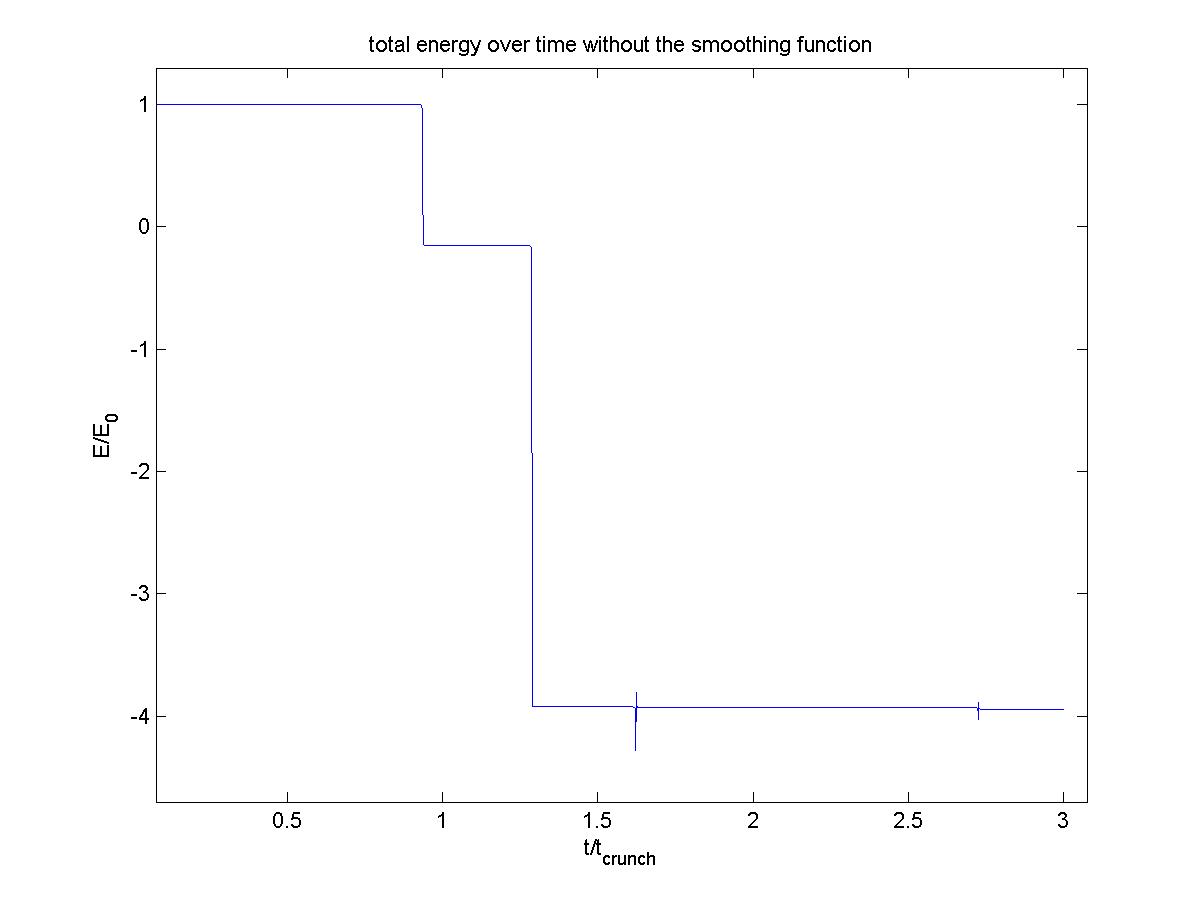
\includegraphics[width=0.8\textwidth]{c1.png}
\end{figure}
\begin{figure}[h]
	\caption{The fraction of particles with positive energy (=ejected particles) as a function of time, without smoothing factor\label{d2}}
	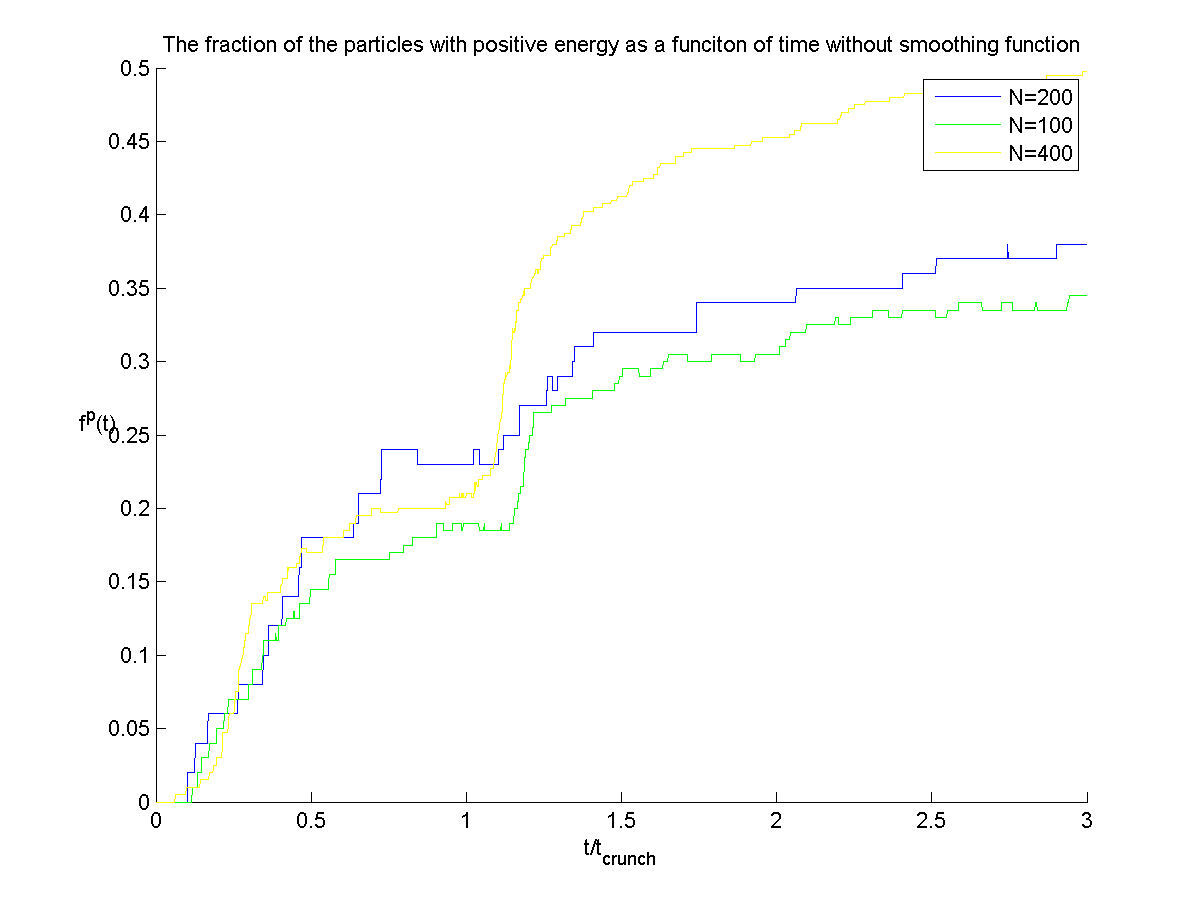
\includegraphics[width=0.8\textwidth]{d2.png}
\end{figure}
\begin{figure}[h]
	\caption{Energy of the system vs particles ejected for $N=100$, without smoothing function\label{d3}}
	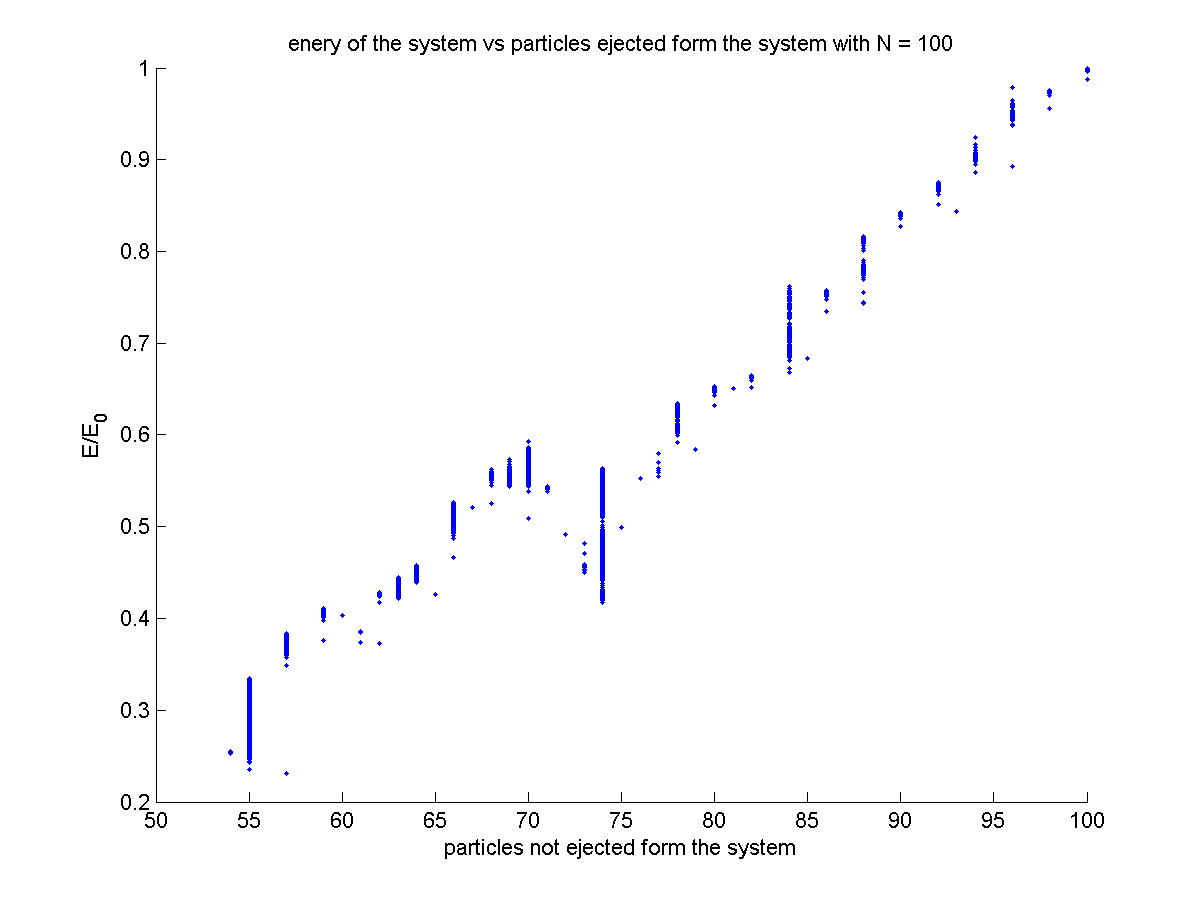
\includegraphics[width=0.8\textwidth]{d3.png}
\end{figure}


The previous results all show one important problem: We do not really conserve energy, as our system is not really realistic when it comes to small distances between two or more particles. Our objects are actually infinitely small mass points instead of bodies with a finite range like stars or planets! This can lead to serious problems. To demonstrate that, we can just take the case of a system with only $N=2$ particles starting at rest. In our model as well as in reality, those two particles would be accelerated towards each other and gain (negative) potential energy in the same way they gain (positive) kinetic energy; but in reality, those particles would, after some time, collide with each other. However, in our model, these particles will never collide as they have no extent! They can get closer and closer, leading to nearly infinitely high forces. In fact, they could even be at the exact same point in space which would imply an infinite force! Together with the finite, non-zero step length in time, these unrealistically high forces can lead to a velocity of the two stars that is high enough to make them unbound! To avoid this, it seems to be reasonable to introduce a smoothing function that guarantees finite forces even for small distances between the objects. This can be justified by the fact that in reality two extended objects cannot get infinitely close as described above. We set up this smoothing factor according to the project instructions by changing the pure Newtonian force in the following way:
\begin{equation}
F_\mathrm{mod}=-\frac{G*M_1*M_2}{r^2+\epsilon^2}
\end{equation}
where $\epsilon$ is a small real constant. We tried many different values of $\epsilon$, ending up with a value of $\epsilon=0.29$ giving us the best energy conservation. To show that, we plotted the total energy of our system again as function of time like we did in fig. \ref{d3}. The new plot in fig.\ref{e1} now looks completely different: We can see that for very short times, we can get high potential energy, but we never reach values lower than the initial energy. Although this diagram covers a time range more than ten times longer than in fig \ref{d3}, we have our energy conserved very well. This is one of the best tests we can implement for our algorithms as we do not have analytical solutions to the $N$-body problem that we can compare our results to! Even the very short peaks in the energy can be explained by our finite step length in time: It can happen that the planets get much closer to each other during one time step while still having the velocity that was calculated based on the force and acceleration of the previous step. As the velocity is somehow \glqq behind\grqq the force in time, we will often observe this behaviour where the potential increases before the velocity (and the kinetic energy) can settle accordingly. That means that we only have long term energy conservation while we can experience some short term peaks due to the finite step length. This long term conservation is delivered very well by our algorithm, justifying our choice of the smoothing factor.

\begin{figure}[h]
	\caption{The total energy of the system over time, with smoothing 		function\label{e1}}
	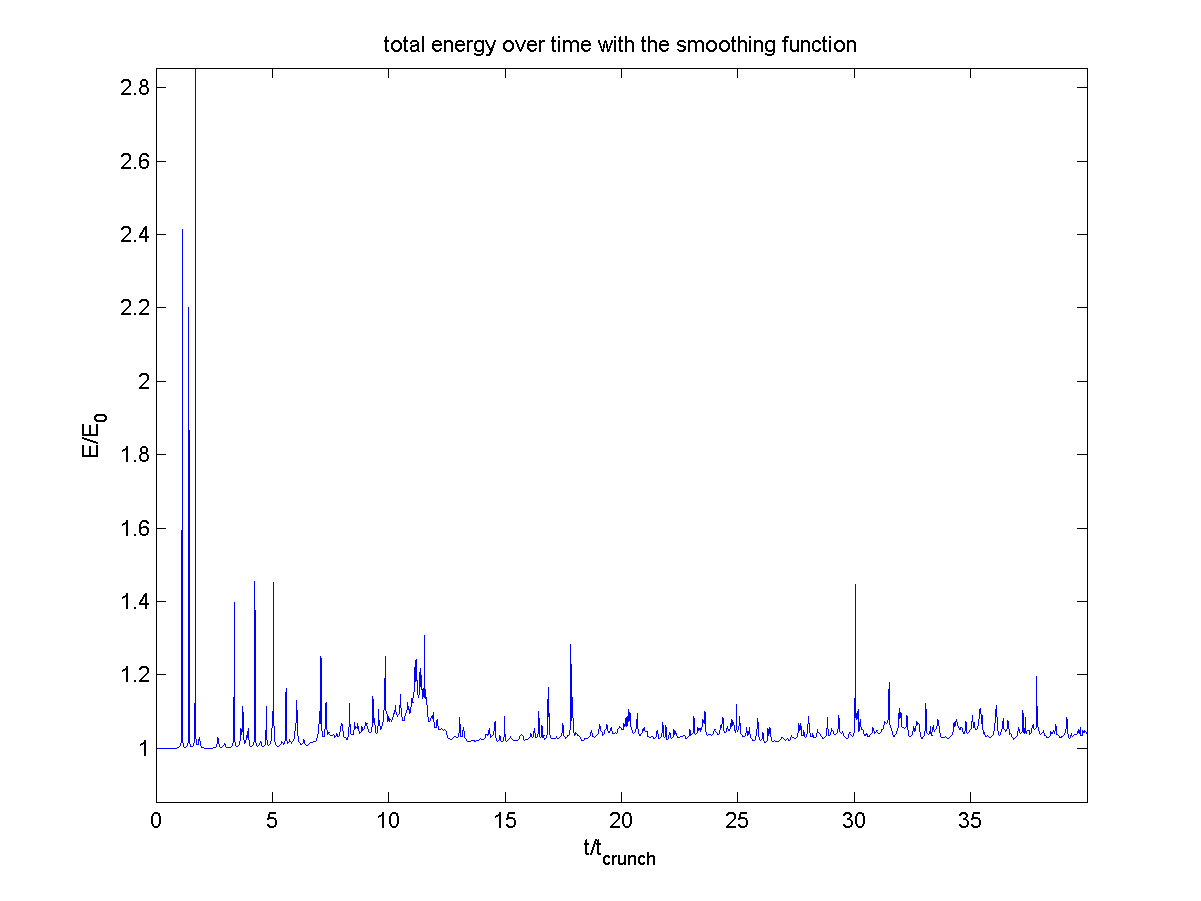
\includegraphics[width=0.8\textwidth]{e1.png}
\end{figure}

An interesting consequence of the newly introduced smoothing function can be seen in fig. \ref{e2}: This is basically the same plot as in fig. \ref{d2}, but now with this new factor. We can see that we now don't have any objects ejected until it comes to the first crunch! After that, many particles get ejected very fast in a way that is very similar to the behaviour that we experienced without smoothing function. Our system seems to be completely stable until it implodes for the first time.

\begin{figure}[h]
	\caption{The fraction of particles with positive energy (=ejected particles) as a function of time, with smoothing factor\label{e2}}
	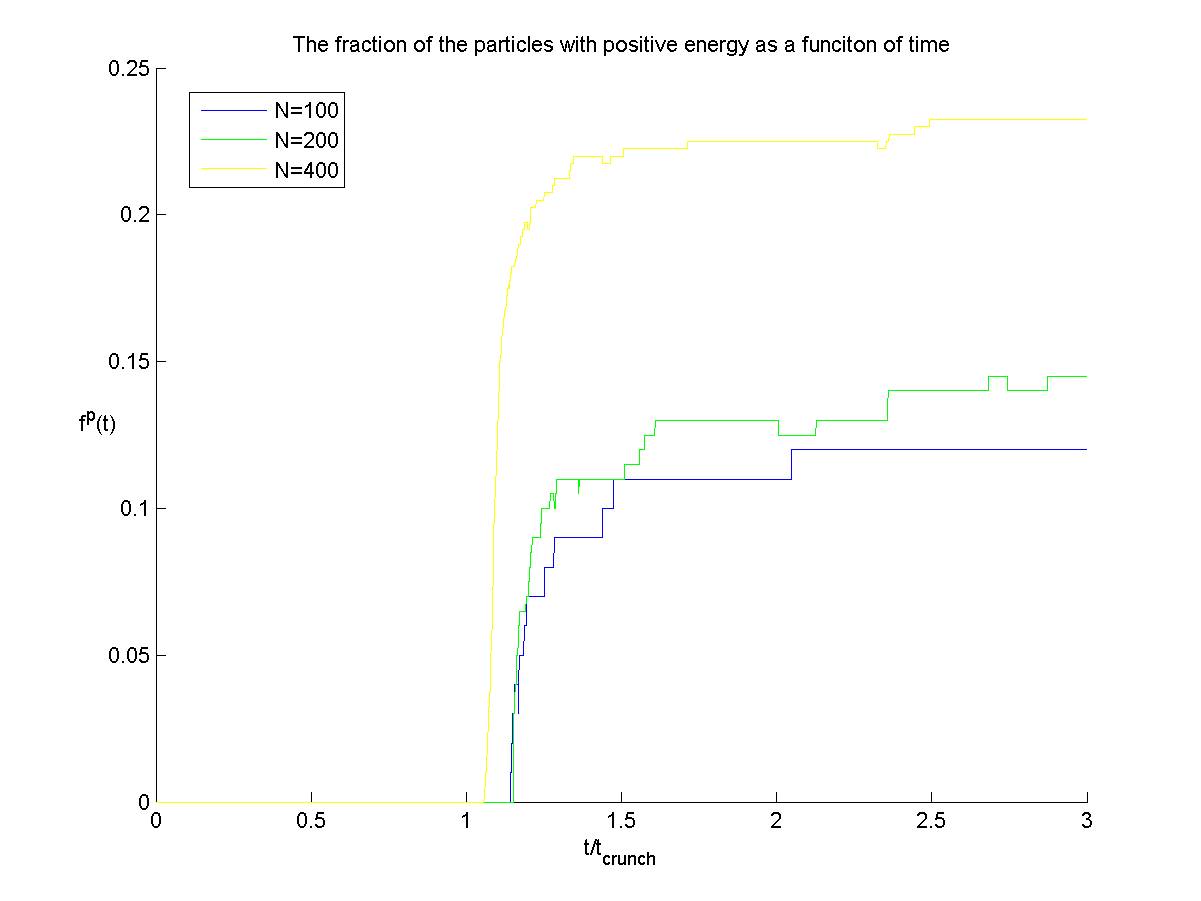
\includegraphics[width=0.8\textwidth]{e2.png}
\end{figure}

As mentioned before, there are not many test we can implement in our $N$-body system due to the lack of analytical solutions. We showed that our algorithm is consistent under the aspect of energy conservation and is able to reproduce a stable system until it crunches for the first time. But there is one more test that we can perform: We can check whether our program is able to validate the virial theorem. This theorem states the following equation for the averages over time of kinetic energy $<K>$ and potential energy $<V>$:
\begin{equation}
2<K>=-<V>
\end{equation}
We plotted the development of the ratio $<V>/<K>$ over time for one system in fig. \ref{f1}. We can clearly see that after a long time, we reach a stable state at $-2$. This is exactly the result that we expected through the virial theorem. This also underlines the exactness of the algorithm.

\begin{figure}[h]
	\caption{Energy of the system vs particles ejected for $N=100$, with smoothing function\label{f1}}
	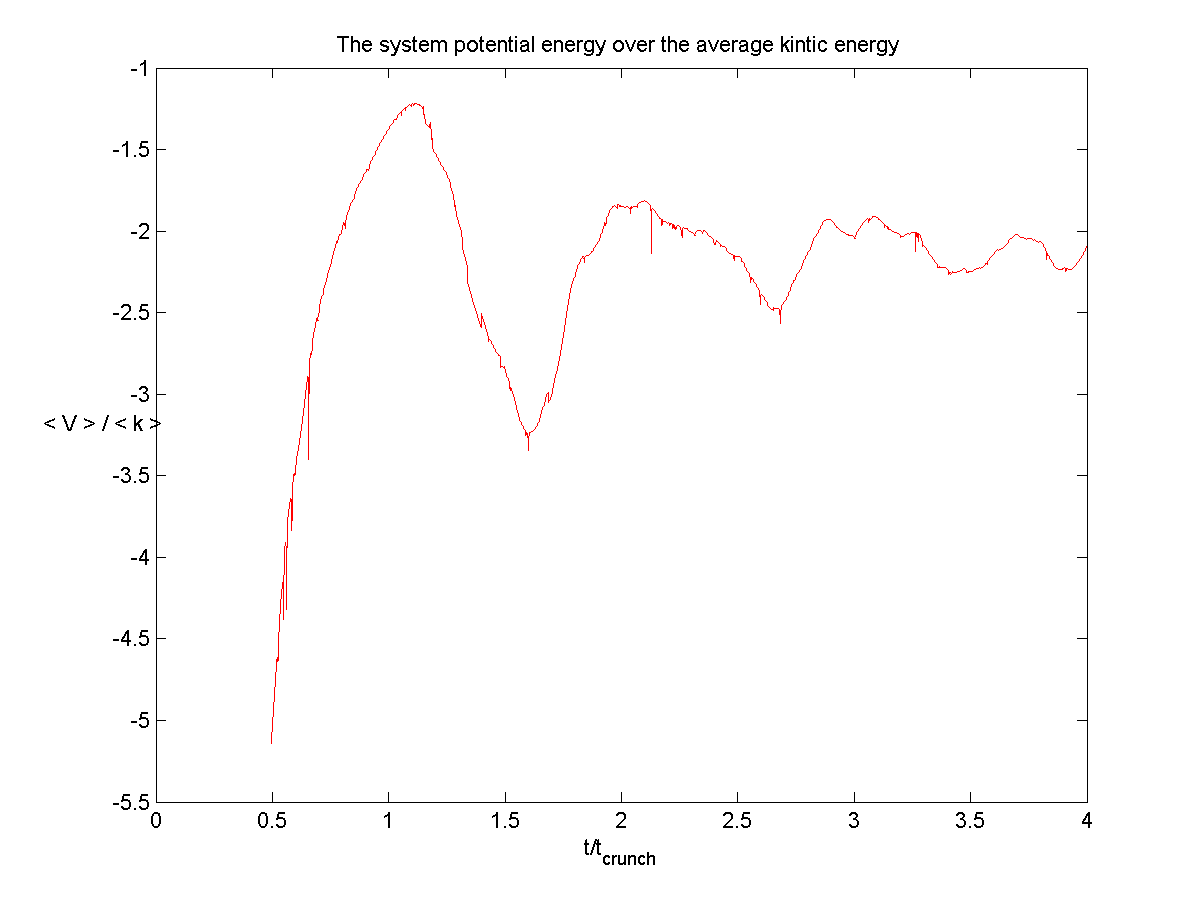
\includegraphics[width=0.8\textwidth]{f1.png}
\end{figure}

\section{Discussion}

\section{Source code}

\end{document}